\documentclass[aspectratio=1610]{beamer}
\usepackage{iftex}
\usepackage{pdfpages}
\ifLuaTeX\else
	\usepackage[utf8]{inputenc}
	\usepackage[T1]{fontenc}
\fi
\usetheme[
% titleimagecolor=red,       % [gray], darkgray, red, blue, green
% titleimagemargin=2mm,      % Distance [2mm]    Frame around title page image
% navigationsymbols=false,   % true   / [false]  Navigation symbols in the foot
% mathseriffont=false,       % true   / [false]  Serif / non-serif math fonts
% foot=true,                 % [true] / false    Footline or not
% nofootslidenum=false       % true   / [false]  Keep slide num even when foot=false
% footlogo=true,             % [true] / false    Put LU logo to the left of footer
% english=true,              % [true] / false    English / Swedish logo
% LTHlogo=false,             % true   / [false]  Use LTH logo instead of LU on title and end pages.
% blackenumeratenumber=true, % [true] / false    Black enumerate numbers, o.w. Lund bronze
% blackitemmark=false,       % true   / [false]  Black item marks, o.w. Lund bronze
% defaultfont=palatino,      % [palatino], beamer, lu
% sectionframe=true,
]{ulund}
%%%%%%%%%%%%%%%%%%%%% Layout commands 
%%%% Foot
% \ulundfootleft{\insertshortauthor}
% \ulundfootmid{\insertshorttitle}
% \ulundfootright{\insertframenumber}% {\insertframenumber:\inserttotalframenumber}
%%%% Titleimage
% \titleimage{Pictures/ULUNDcolor} % Replaces the LU image. Voids option titleimagecolor
%%%%%%%%%%%%%%%%%%%%%%%%%%%%%%%%%%%

\usepackage{listcode}

\newcommand{\code}[1]{\lstinline{#1}}

\title[JavaScript]{HTML and CSS}
\author[EDAF90]{%
  EDAF90 Web Programming\newline
  Per Andersson}
%%%%%%%%%%%%%%%%%%%%%
%\usepackage{verbatim}
%%%%%%%%%%%%% Verbatim code box
\usepackage[skins,listings]{tcolorbox}
\ifLuaTeX\else
	\tcbuselibrary{listingsutf8}
\fi
\newtcblisting{CodeBox}[2][]{% Only code
  colframe=black,
  colback=white,
  arc=1pt,
  boxrule=0.5pt,
  top=0mm,bottom=0pt,left=0pt,
  colbacktitle=gray!40,
  coltitle=black,
  fonttitle=\sffamily,
  listing only,
  hbox,
  listing options={
    basicstyle=\small\ttfamily,
    breaklines=true,
    columns=fullflexible,
    language=Java,
    basicstyle = \ttfamily,
    showstringspaces=false,
    morekeywords= {undefined, NaN, function, export, var, let}
  },
  title=#2,#1
}

\lstset{
    basicstyle=\small\ttfamily,
    breaklines=true,
    columns=fullflexible,
    language=Java,
    basicstyle = \ttfamily,
    showstringspaces=false,
    morekeywords= {undefined, NaN, function, export, var, let}
}

%%%%%%%%%%%%%%%%%%%%%
%%%%%%%%%%%%%%%%%%%%%
%%%%%%%%%%%%%%%%%%%%%

\begin{document}
\begin{frame}[plain]% Use plain to suppress footline box
  \titlepage
\end{frame}

%--------------------
\frame{
    \frametitle{Outline}
    \tableofcontents%[subsectionstyle=hide]%[currentsection,currentsubsection]
}

%---HTML ---------------------------------------------------
\section{Internet and Terminology}

%---------------------------------------------------------------------------------
\begin{frame}[fragile]
\frametitle{Terminologi}
\color{structure}
\begin{itemize}\color{structure}
  \item client-server (backend-frontend)
  \item static web page
  \item dynamic web page
  \item Content Management Systems (CMS), for example WordPress, Drupal, and Joomla
  \item singel page web application
  \item Web Application Frameworks
  \item responsive design
  \item universal design
\end{itemize}
\end{frame}

%---------------------------------------------------------------------------------
\begin{frame}[fragile]
\frametitle{Terminologi}
\color{structure}
\end{frame}

%---------------------------------------------------------------------------------
\begin{frame}[fragile]
\frametitle{Standardisering}
\color{structure}
\begin{itemize}\color{structure}
  \item Internet Engineering Task Force (IETF) - RFC and "rough consensus and running code"
  \item World Wide Web Consortium (W3C)
  \item European Computer Manufacturers Association (ECMA) and ECMAScript
\end{itemize}
\end{frame}

\section{Character encoding}

%---------------------------------------------------------------------------------
\begin{frame}
\frametitle{Locales and Word Order}
\color{structure}
Text communicate infomation to the user. To handle text in a program you need:
\begin{itemize}
  \item encoding --- A mapping (value $ \leftrightarrow $ symbol)
  \item locale --- How to render dates, digits and time depends on where you are:
  \begin{itemize}
    \item Digits: 3.142 or 3,142?
    \item Date: 01/02/03
    \begin{itemize}\color{structure}
      \item 3 februari 2001?
      \item January 2, 2003?
      \item 1 February 2003?
    \end{itemize}
  \end{itemize}
  \item collation --- character order. Is Andersson before or after Åkesson?
\end{itemize}
\end{frame}

%---------------------------------------------------------------------------------
\begin{frame}[fragile]
\frametitle{Character encoding}
\color{structure}
There exists many different ways to encode characters
\begin{itemize}\color{structure}
  \item fixed width
  \item variable width (compare to Hoffman coding)
\end{itemize}
Some common standards:
\begin{itemize}\color{structure}
  \item Unicode and utf8, no just encoding, also collation (sorting)
  \item ISO-8859-1/latin 1
  \item UTF8 is conquering the world, it is standard for Java och JavaScript.
\end{itemize}
\end{frame}

%---------------------------------------------------------------------------------
\begin{frame}[fragile]
\frametitle{Unicode}
\color{structure}
A standard including:
\begin{itemize}\color{structure}
  \item visual reference
  \item set of standard character encodings
  \item an encoding method
  \item character properties (lower/upper case)
  \item rules for normalization, decomposition, collation
  \item rules for rendering, and bidirectional text display order (right-to-left, left-to-right scripts)
\end{itemize}
\end{frame}

\begin{frame}
\frametitle{Unicode Blocks (Simplified)}
\color{structure}
\begin{footnotesize}
\begin{table}
\begin{center}
\begin{tabular}{llll}
\hline
\textbf{Code}& \textbf{Name}& \textbf{Code}& \textbf{Name} \\
\hline
U+0000& Basic Latin& U+1400& Unified Canadian Aboriginal Syllabic \\
%\hline
U+0080& Latin-1 Supplement& U+1680& Ogham, Runic \\
%\hline
U+0100& Latin Extended-A& U+1780& Khmer \\
%\hline
U+0180& Latin Extended-B& U+1800& Mongolian \\
%\hline
U+0250& IPA Extensions& U+1E00& Latin Extended Additional \\
%\hline
U+02B0& Spacing Modifier Letters& U+1F00& Extended Greek  \\
%\hline
U+0300& Combining Diacritical Marks& U+2000& Symbols \\
%\hline
U+0370& Greek& U+2800& Braille Patterns \\
%\hline
U+0400& Cyrillic& U+2E80& CJK Radicals Supplement \\
%\hline
U+0530& Armenian& U+2F80& KangXi Radicals \\
%\hline
U+0590& Hebrew& U+3000& CJK Symbols and Punctuation \\
%\hline
U+0600& Arabic& U+3040& Hiragana, Katakana \\
%\hline
U+0700& Syriac& U+3100& Bopomofo \\
%\hline
U+0780& Thaana& U+3130& Hangul Compatibility Jamo \\
\hline
\end{tabular}
\end{center}
\end{table}
\end{footnotesize}
\end{frame}

\begin{frame}
\frametitle{Unicode Blocks (Simplified) (II)}
\color{structure}
\begin{footnotesize}
\begin{table}
\begin{center}
\begin{tabular}{llll}
\hline
\textbf{Code}& \textbf{Name}& \textbf{Code}& \textbf{Name} \\
\hline
%\hline
U+0900& Devanagari, Bengali& U+3190& Kanbun \\
%\hline
U+0A00& Gurmukhi, Gujarati& U+31A0& Bopomofo Extended \\
%\hline
U+0B00& Oriya, Tamil& U+3200& Enclosed CJK Letters and Months \\
%\hline
U+0C00& Telugu, Kannada& U+3300& CJK Compatibility \\
%\hline
U+0D00& Malayalam, Sinhala& U+3400& CJK Unified Ideographs Extension A \\
%\hline
U+0E00& Thai, Lao& U+4E00& CJK Unified Ideographs \\
%\hline
U+0F00& Tibetan& U+A000& Yi Syllables \\
%\hline
U+1000& Myanmar& U+A490& Yi Radicals \\
%\hline
U+10A0& Georgian& U+AC00& Hangul Syllables \\
%\hline
U+1100& Hangul Jamo& U+D800& Surrogates \\
%\hline
U+1200& Ethiopic& U+E000& Private Use \\
%\hline
U+13A0& Cherokee& U+F900& Others \\
\hline
\end{tabular}
\end{center}
\end{table}
\end{footnotesize}
\end{frame}

\begin{frame}[fragile]
\frametitle{The Unicode Encoding Schemes}
\color{structure}
\begin{itemize}
\item each character have a unique unicode
\item different ways to store the unique unicodes in a file:
  \begin{itemize}
    \item UTF-8, UTF-16, and UTF-32.\\
  \end{itemize}
\item UTF-16 used to be standard\\
\item uses 16 bits per character – 2 bytes –\\
\item \textit{FÊTE} \verb=0046 00CA 0054 0045=\\
\item UTF-8 has variable length for each character\\
\end{itemize}
\end{frame}

\begin{frame}
\frametitle{UTF-8}
\color{structure}
\begin{center}
\begin{tabular}{rl}
\hline
\multicolumn{1}{l}{\textbf{Range}}& \textbf{Encoding} \\
\hline
U-0000 -- U-007F& 0xxxxxxx \\
%\hline
U-0080 -- U-07FF& 110xxxxx 10xxxxxx \\
%\hline
U-0800 -- U-FFFF& 1110xxxx 10xxxxxx 10xxxxxx \\
%\hline
U-010000 -- U-10FFFF& 11110xxx 10xxxxxx 10xxxxxx 10xxxxxx \\
\hline
\end{tabular}
\end{center}
\end{frame}

\section{HTML}

%---------------------------------------------------------------------------------
\begin{frame}[fragile]
\frametitle{HTML}
\begin{lstlisting}[style=htmlcssjs]
<!DOCTYPE html>
<html>
  <head>
    <meta charset="utf-8">
    <title>Hello World</title>
    <link rel="stylesheet" href="css/styles.css">
    <script src="my-awsome-code.js"></script>
    <base  href="https://www.cs.lth.se/eda095/">
  </head>

  <body>
    <h1>Hello World</h1>
    <p id="my-blue-box">My awsome page.
  </body>
</html>
\end{lstlisting}
\end{frame}

%---------------------------------------------------------------------------------
\begin{frame}[fragile]
\frametitle{HTML - element}

Semantic tags\\
\html{<h1>, <h2>, <p>,  <abbr>, <code>, <samp>, <kbd>, <var>, <footer>, <header>, <details>, <nav>}\ldots
\bigskip

Structure\\
\html{<table>, <ul>, <ol>, <div>, <span>}\ldots
\bigskip

Functionality included\\
\html{<form>, <input>, <select>, <button>, <a>}\ldots
\bigskip
\color{structure}

För att lära dig mer om HTML-taggar se \url{https://www.w3schools.com/tags/default.asp}
\end{frame}

%---------------------------------------------------------------------------------
\begin{frame}[fragile]
\frametitle{HTML - elements}
\color{structure}
Data:
\begin{itemize}\color{structure}
\item between the tags: \html{<h1>My Headline</h1>}
  \begin{itemize}\color{structure}
  \item is rendered
  \item text 
  \item may include other html-elements 
  \end{itemize}
\end{itemize}

\begin{itemize}\color{structure}
\item attributes: \html{<a href="http://cs.lth.se">my link</a>} 
  \begin{itemize}\color{structure}
    \item text is not shown on screen
    \item only text
  \end{itemize}
  \item \html{id} - optional attribute, unique for each element\\ can be used to find/refer to an element
  \item \html{class} - used for styling (do not relate to JavaScript classes)
\end{itemize}
\bigskip
tag + content $\approx$ element

\end{frame}

\section{Layout}

%---------------------------------------------------------------------------------
\begin{frame}[fragile]
\frametitle{Layout}
\color{structure}
Rendering
\begin{itemize}\color{structure}
\item the rendering is controlled by
\begin{itemize}
  \item element tag: \html{<p>, <select>}
  \item properties: \html{font-family, background-color}
\end{itemize} 
\item some properties are dynamic, updated by the browser rendering engine
\item most properties are inherited from the surrounding
\item properties can not be deleted, only shadowed
\item give an property a value:
\begin{itemize}\color{structure}
  \item the \html{style} attributet in the HTML element
  \item Cascading Style Sheets (CSS)
  \end{itemize}
\end{itemize}

\bigskip
\href{https://www.w3schools.com/css/css_intro.asp}{example of what you can do with css: https://www.w3schools.com/css/css\_intro.asp}
\end{frame}

%---------------------------------------------------------------------------------
\begin{frame}[fragile]
\frametitle{CSS}
\color{structure}
Cascading Style Sheets
\begin{itemize}\color{structure}
\item separate the content from the layout
\item a set of rules:
\begin{itemize}\color{structure}
  \item  selection
  \item declaration (attribut = value)
\end{itemize}
\item the declaration is applied to all elements matching the selection
\end{itemize}
syntax:\\ \code{urval : \{ property1: value1; property2: value2;\}}
\end{frame}

%---------------------------------------------------------------------------------
\begin{frame}[fragile]
\frametitle{CSS - selection}
\color{structure}
CSS selection is based on pattern matching:\\
\begin{itemize}\color{structure}
\item instances of an element: \html{<h1>}
\item all elements with a class: \html{<div class="my-style">}
\item the element with a given \tt{id}: \html{<div id="my-tag">}
\item pseudo classes \html{focus, hover, visited, valid, ...}
\item pseudo element \html{nth-child(2), only-child, ...} 
\item attribute value: \html{[title~="flower"], ...} 
\end{itemize}
Match patterns can be combined
\end{frame}

%---------------------------------------------------------------------------------
\begin{frame}[fragile]
\frametitle{CSS - exempel}
\color{structure}
Example:
\begin{lstlisting}[style=htmlcssjs]
// element
div { color: blue; border: 1px; }
// id, <p id="my-blue-box">
#my-blue-box { background-color: lightblue; }
// class, <div class="center">
.center { text-align: center; color: red; }
// element och and, <p class="center">
p.center { text-align: center; color: green; }
// inside
div p { text-align: center; color: green; }
// all p with a parent div
div > p { text-align: center; color: green; }
// directly after
div + p { text-align: center; color: green; }
// pseudo-class
a:hover { background-color: lightblue; }
\end{lstlisting}
\end{frame}

%---------------------------------------------------------------------------------
\begin{frame}[fragile]
\frametitle{Box Modellen}
\color{structure}
  \centering
  
\includegraphics[width=10cm]{img/box_model}

\end{frame}

%---------------------------------------------------------------------------------
\begin{frame}[fragile]
\frametitle{Layout}
\color{structure}
CSS Properties for layout
\begin{itemize}
  \item \code{display}: \code{block, inline, none, flex, ...}
  \item \code{visibility}: \code{visible, hidden, ...}
  \item \code{position}: \code{static, relative, absolute, fixed, ...}
  \item \code{overflow}: \code{visible, hidden, scroll, auto, ...}
  \item \code{z-index}: \code{auto}, \it{number}
\end{itemize}
\end{frame}

%---------------------------------------------------------------------------------
\begin{frame}[fragile]
\frametitle{Frameworks}
\color{structure}
Creating a good layout is costly. 
\begin{itemize}\color{structure}
  \item needs a lot of testing on different browsers
  \item you can use or extend use existing:
  \begin{itemize}
    \item bootstrap
    \item material design
  \end{itemize}
\end{itemize}
\end{frame}

%---------------------------------------------------------------------------------
\begin{frame}[fragile]
\frametitle{My own standard}
\color{structure}
Each browser have their own implementation of the
\begin{itemize}\color{structure}
  \item rendering engine
  \item JavaScript engine
\end{itemize}
\vspace{5mm}
With their own
\begin{itemize}\color{structure}
  \item interpretation of the standard
  \item selection of standard features to support
  \item bugs
  \item extensions
\end{itemize}
\end{frame}

%---------------------------------------------------------------------------------
\begin{frame}[fragile]
\frametitle{Webkit Mozilla}
\color{structure}
The same feature apperas with different names in different browsers:
\begin{itemize}\color{structure}
  \item \code{box-shadow}
  \item \code{-webkit-box-shadow}
  \item \code{-moz-box-shadow}
\end{itemize}
\end{frame}


\section{Document Object Model}

%---------------------------------------------------------------------------------
\begin{frame}[fragile]
\frametitle{DOM}
\color{structure}
Document Object Model\\
\begin{itemize}\color{structure}
  \item a web page/html is a tree
  \item the nodes are the HTML elements
  \item HTML attriburtes are attributes in the nodes
  \item \html{<html>} is the root of the tree
\end{itemize}
\end{frame}

%---------------------------------------------------------------------------------
\begin{frame}[fragile]
\frametitle{DOM}
\color{structure}
Document Object Model\\
\begin{itemize}\color{structure}
\item \html{Document} is a class for representing the DOM
\item the nodes inherits from the \html{Element.prototype} object
\item the globala variable \code{document} refers to the DOM
\item API for
  \begin{itemize}
    \item navigate in the tree: \code{document.body.getElementsByTagName( 'H1' )}
    \item serach for elements: \code{document.getElementById("intro")}
    \item modify the DOM: \code{Element.innerHTML}
    \item read/writer attribute, \code{myInputElement.value="Nisse Hult"}
  \end{itemize}
\end{itemize}
\end{frame}

%---------------------------------------------------------------------------------
\begin{frame}[fragile]
\frametitle{Events}
\color{structure}

\begin{itemize}\color{structure}
\item the browser creates events: \code{blur, submit, resize, keydown}
\item call-back-methods
\begin{itemize}
  \item \code{<p id="demo" onclick="myHandler(event)">}
  \item \code{addEventListener(eventType, handler[, options])}
\end{itemize}
\item \code{event} is an instance of \code{Event}
\item event propagates trough the DOMen, three phases:
  \begin{enumerate}
    \item capturing
    \item target
    \item bubbling
  \end{enumerate}
\end{itemize}

\end{frame}

%---------------------------------------------------------------------------------
\begin{frame}[fragile]
\frametitle{event phases}
\color{structure}
  \centering
  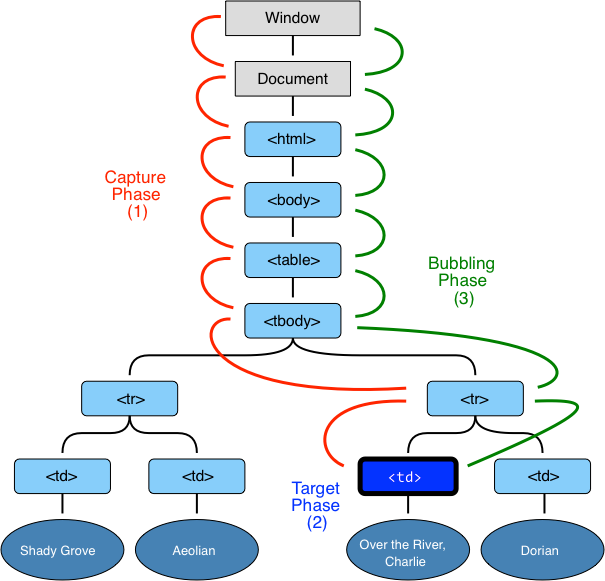
\includegraphics[width=8cm]{img/eventflow}

\end{frame}

%---------------------------------------------------------------------------------
\begin{frame}[fragile]
\frametitle{Events}
\color{structure}

\begin{itemize}\color{structure}
\item not all events propagate, \code{focus} do not.
\item \code{this}===\code{event.currentTarget}, the DOM element containing the handler
\item \code{event.target} the source of the event, a DOM element
\item event propagates trough the DOMen, three phases:
  \begin{enumerate}
    \item capturing
    \item target
    \item bubbling
  \end{enumerate}
\item \code{event.stopPropagation()}
\item \code{event.preventDefault()}
\end{itemize}

\end{frame}

%---------------------------------------------------------------------------------
\begin{frame}[fragile]
\frametitle{Forms}
\color{structure}

\begin{lstlisting}[style=htmlcssjs]
<form onsubmit="myFunction(event)">
  <label for="id-checkbox">Checkbox:</label>
  <input type="checkbox" id="id-checkbox"/>
  <input type="submit" value="Send Request">
</form>
\end{lstlisting}

Form submission is default behaviour for many events (click on submit button, enter in input field)
\begin{itemize}
  \item submit the form using HTTP
  \item the server responds with a new html-page
  \item the browser renders the new page
\end{itemize}

\end{frame}



%%%%%%%%%%%
\end{document}
